\documentclass{standalone}
\usepackage{tikz}
\usepackage{textcomp}

\begin{document}

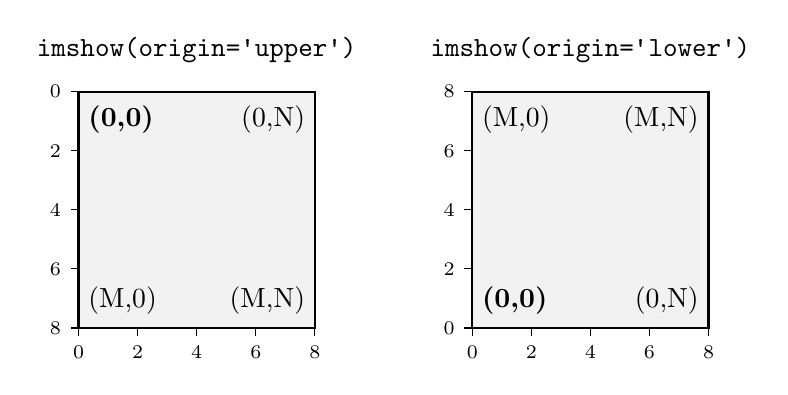
\begin{tikzpicture}

% origin = upper
\draw [thick, fill=gray, fill opacity=0.1] (0,0) -- (3,0) -- (3,3) -- (0,3) -- cycle;
\node [above] at (1.5,3.25) {\texttt{imshow(origin=\textquotesingle upper\textquotesingle )}};
\foreach \x / \t in {0/0, 0.75/2, 1.5/4, 2.25/6, 3/8}{
    \draw (\x,0) -- (\x,-0.1);
    \node [below] at (\x,-0.1) {\scriptsize \t};
}

\foreach \y / \t in {0/8, 0.75/6, 1.5/4, 2.25/2, 3/0}{
    \draw (0,\y) -- (-0.1,\y);
    \node [left] at (-0.1,\y) {\scriptsize \t};
}

\node [right] at (0,2.65) {\textbf{(0,0)}};
\node [left] at (3,2.65) {(0,N)};
\node [right] at (0,0.35) {(M,0)};
\node [left] at (3,0.35) {(M,N)};

% origin = lower
\draw [thick, fill=gray, fill opacity=0.1] (5,0) -- (5,3) -- (8,3) -- (8,0) -- cycle;
\node [above] at (6.5,3.25) {\texttt{imshow(origin=\textquotesingle lower\textquotesingle )}};
\foreach \x / \t in {5/0, 5.75/2, 6.5/4, 7.25/6, 8/8}{
    \draw (\x,0) -- (\x,-0.1);
    \node [below] at (\x,-0.1) {\scriptsize \t};
}

\foreach \y / \t in {0/0, 0.75/2, 1.5/4, 2.25/6, 3/8}{
    \draw (5,\y) -- (4.9,\y);
    \node [left] at (4.9,\y) {\scriptsize \t};
}

\node [right] at (5,2.65) {(M,0)};
\node [left] at (8,2.65) {(M,N)};
\node [right] at (5,0.35) {\textbf{(0,0)}};
\node [left] at (8,0.35) {(0,N)};


\end{tikzpicture}
\end{document}
